\documentclass[10pt,twocolumn]{article}
\usepackage[T1]{fontenc}
\usepackage[utf8]{inputenc}
\usepackage[margin=0.75in]{geometry}
\usepackage{times}
\usepackage{microtype}
\usepackage{graphicx}
\usepackage{booktabs}
\usepackage{enumitem}
\usepackage{amsmath}
\usepackage{amssymb}
\usepackage{hyperref}
\usepackage{array}
\usepackage{titlesec}
\usepackage{tikz}
\usepackage{pgfplots}
\usepackage{caption}
\usepackage{listings}
\usetikzlibrary{arrows.meta,positioning,shapes.geometric,fit,backgrounds}
\pgfplotsset{compat=1.18}

\definecolor{recallblue}{RGB}{47,111,191}
\definecolor{reductiongreen}{RGB}{57,140,88}
\definecolor{precisionorange}{RGB}{211,125,44}
\definecolor{fiviolet}{RGB}{126,87,194}

\tikzset{
  stage/.style={draw, rounded corners=3pt, thick, align=center,
                minimum height=1.6cm, minimum width=2.8cm, fill=blue!8},
  mini/.style={draw, rounded corners=2pt, align=left,
               fill=gray!5, inner sep=6pt},
  flowarrow/.style={-{Latex[length=3mm]}, thick},
  evidence/.style={draw, rounded corners=3pt, align=center,
                   fill=green!10, minimum width=2.2cm, minimum height=0.75cm},
  entitybox/.style={draw, rounded corners=3pt, align=left,
                    fill=gray!4, inner sep=5pt, text width=0.34\textwidth}
}

\titleformat{\section}{\large\bfseries}{\thesection.}{0.5em}{}
\titleformat{\subsection}{\normalsize\bfseries}{\thesubsection.}{0.4em}{}
\captionsetup{font=small, labelfont=bf}
\setlength{\parskip}{0.35em}
\setlength{\parindent}{0pt}
\setlength{\columnsep}{0.28in}
\setlength{\columnseprule}{0pt}
\setlength{\emergencystretch}{2em}
\raggedbottom
\setlist[itemize]{leftmargin=*,topsep=2pt,itemsep=1pt}

\title{A CPU-First Entity Resolution Pipeline\\
       with Witness-Driven Candidate Reduction}
\author{
  Noureddine Mohammedi \and Azouaou Zouaoui \and
  Massizelle Boubadjou \and Nour Khelassi \and Aya Chihoub
}
\date{April 2026 --- Université Paris Cité}

\begin{document}
\maketitle

\begin{abstract}
We present an end-to-end entity resolution (ER) pipeline for heterogeneous
benchmark datasets. The pipeline follows a four-stage architecture---ingestion,
blocking, matching, and clustering---built around a single
witness-driven candidate-generation strategy called
\texttt{cw\_semantic\_predictive}. The key design goal is to remain CPU-first
by aggressively collapsing the candidate search space before expensive
semantic matching. Experiments on three standard benchmarks show that strong
symbolic reduction combined with bounded semantic and predictive rescue
achieves high candidate recall (up to 95.5\%) while eliminating more than
99\% of the Cartesian product, leading to competitive end-to-end F1 scores
across product and bibliographic domains.
\end{abstract}

\section{Introduction}
Entity resolution (ER) is the task of identifying records from one or more
data sources that refer to the same real-world object. It arises in
e-commerce (matching products across catalogs), bibliographic databases
(deduplicating publications), and knowledge graph construction (linking
entities across RDF sources). Unresolved duplicates degrade the quality of
downstream analytics, search, and data integration.

The core difficulty of ER is representation mismatch: two records describing
the same entity may differ in formatting, abbreviations, attribute order,
or spelling. Even when matching is conceptually simple, the brute-force
search space is the Cartesian product $S_1 \times S_2$, which grows
quadratically and quickly becomes impractical. Candidate reduction is
therefore a central systems challenge.

Our project targets four competing objectives simultaneously:
\begin{itemize}
  \item high recall of true matches after candidate generation,
  \item strong reduction of the explicit comparison space,
  \item dataset-generic design without benchmark-specific branches,
  \item practical CPU-first execution on commodity hardware.
\end{itemize}

The main research contribution is a \emph{witness-driven} candidate
strategy that departs from a purely pair-centric workflow. Rather than
enumerating pairs and then pruning them, the system first extracts
heterogeneous evidence signals (\emph{witnesses}) for each entity, collapses
compatible evidence regions across sources, and materializes explicit pairs
only when the residual ambiguity is small. Semantic and predictive rescues
are applied afterwards, bounded to entities that symbolic evidence alone
could not resolve.

\begin{figure*}[t]
\centering
\resizebox{\textwidth}{!}{%
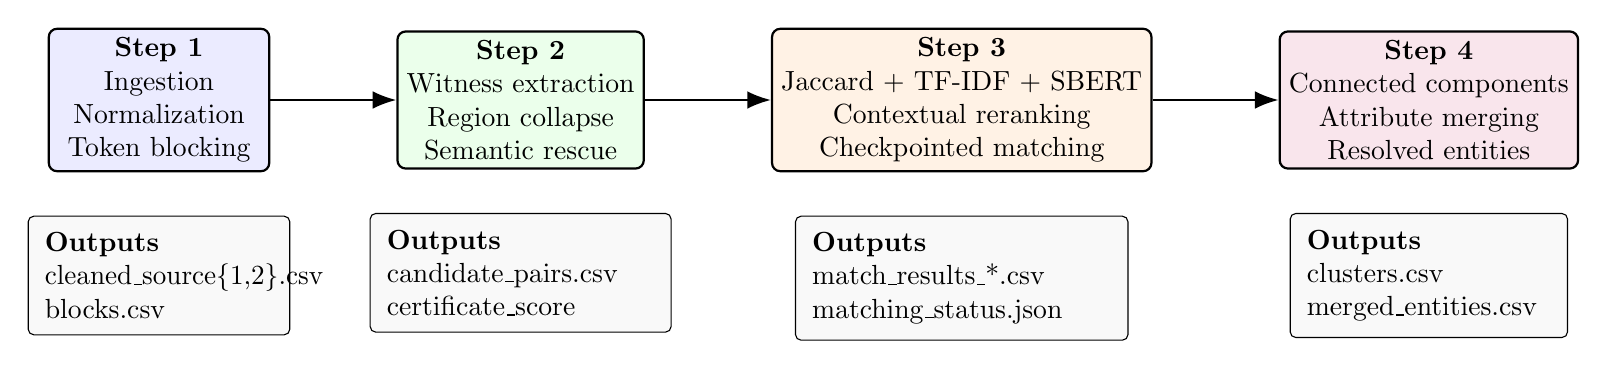
\begin{tikzpicture}[node distance=1.6cm]
  \node[stage] (m1)
    {\textbf{Step 1}\\Ingestion\\Normalization\\Token blocking};
  \node[stage, right=of m1, fill=green!8] (m2)
    {\textbf{Step 2}\\Witness extraction\\Region collapse\\Semantic rescue};
  \node[stage, right=of m2, fill=orange!10] (m3)
    {\textbf{Step 3}\\Jaccard + TF-IDF + SBERT\\Contextual reranking\\Checkpointed matching};
  \node[stage, right=of m3, fill=purple!10] (m4)
    {\textbf{Step 4}\\Connected components\\Attribute merging\\Resolved entities};
  \draw[flowarrow] (m1) -- (m2);
  \draw[flowarrow] (m2) -- (m3);
  \draw[flowarrow] (m3) -- (m4);
  \node[mini, below=0.55cm of m1, text width=2.9cm]
    {\textbf{Outputs}\\cleaned\_source\{1,2\}.csv\\blocks.csv};
  \node[mini, below=0.55cm of m2, text width=3.4cm]
    {\textbf{Outputs}\\candidate\_pairs.csv\\certificate\_score};
  \node[mini, below=0.55cm of m3, text width=3.8cm]
    {\textbf{Outputs}\\match\_results\_*.csv\\matching\_status.json};
  \node[mini, below=0.55cm of m4, text width=3.1cm]
    {\textbf{Outputs}\\clusters.csv\\merged\_entities.csv};
\end{tikzpicture}}
\caption{End-to-end pipeline. Each step produces explicit intermediate
  artifacts, enabling partial reruns, inspection, and resumable matching.}
\label{fig:workflow}
\end{figure*}

\begin{figure*}[t]
\centering
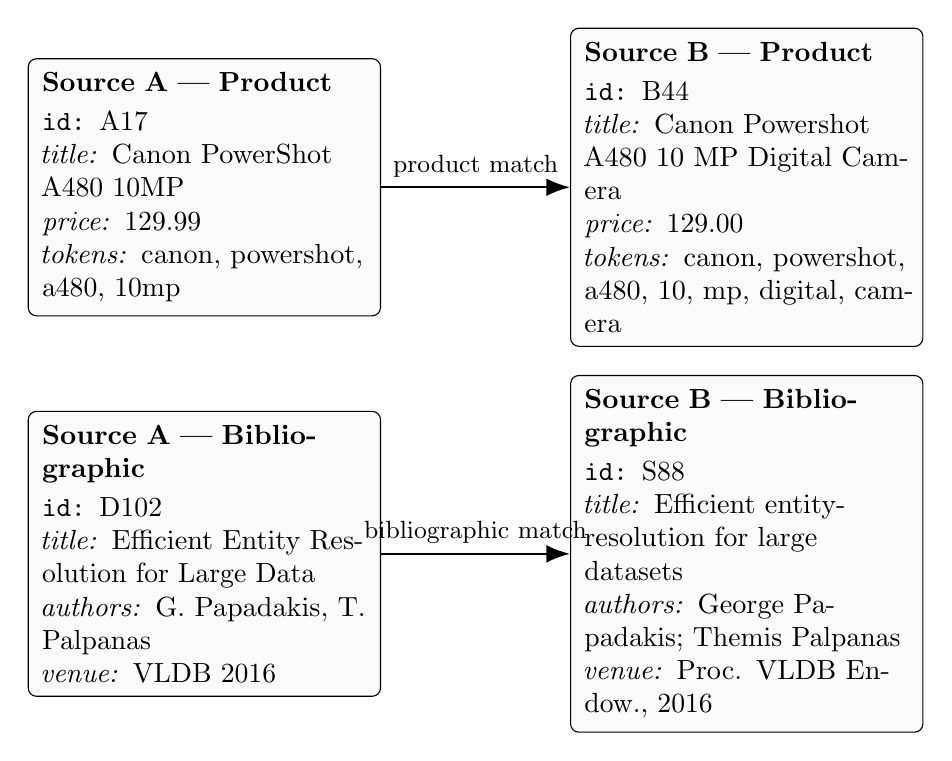
\begin{tikzpicture}[node distance=1.3cm]
  \node[entitybox] (prodA) {
    \textbf{Source A — Product}\\[2pt]
    \texttt{id:} A17\\
    \textit{title:} Canon PowerShot A480 10MP\\
    \textit{price:} 129.99\\
    \textit{tokens:} canon, powershot, a480, 10mp
  };
  \node[entitybox, right=2.4cm of prodA] (prodB) {
    \textbf{Source B — Product}\\[2pt]
    \texttt{id:} B44\\
    \textit{title:} Canon Powershot A480 10 MP Digital Camera\\
    \textit{price:} 129.00\\
    \textit{tokens:} canon, powershot, a480, 10, mp, digital, camera
  };
  \node[entitybox, below=1.2cm of prodA] (bibA) {
    \textbf{Source A — Bibliographic}\\[2pt]
    \texttt{id:} D102\\
    \textit{title:} Efficient Entity Resolution for Large Data\\
    \textit{authors:} G. Papadakis, T. Palpanas\\
    \textit{venue:} VLDB 2016
  };
  \node[entitybox, right=2.4cm of bibA] (bibB) {
    \textbf{Source B — Bibliographic}\\[2pt]
    \texttt{id:} S88\\
    \textit{title:} Efficient entity-resolution for large datasets\\
    \textit{authors:} George Papadakis; Themis Palpanas\\
    \textit{venue:} Proc. VLDB Endow., 2016
  };
  \draw[flowarrow, thick] (prodA.east)
    -- node[above]{\small product match} (prodB.west);
  \draw[flowarrow, thick] (bibA.east)
    -- node[above]{\small bibliographic match} (bibB.west);
\end{tikzpicture}
\caption{Illustrative ER pairs used throughout the paper. Neither pair is
  textually identical, yet both share enough lexical, structural, and
  semantic evidence to survive candidate reduction and rank as final matches.}
\label{fig:examplepair}
\end{figure*}

\section{Related Work}

\textbf{End-to-end ER pipelines.}
Christophides et al.~\cite{christophides2021survey} provide a comprehensive
survey of ER for big data, framing the problem as a coupled pipeline of
cleaning, blocking, matching, and clustering. Our project follows this
decomposition directly, with each step corresponding to one
survey-level task. The key difference is that our implementation shifts
emphasis toward compressing the candidate space before matching rather than
relying on a more expensive scorer.

\textbf{Approximate blocking and meta-blocking.}
Papadakis et al.~\cite{papadakis2016blocking} analyse approximate blocking
strategies and their impact on recall and reduction. Their analysis motivated
our focus on strong pre-matching candidate reduction. Our Step 2 stage goes
one step further: instead of pruning an already-materialised pair graph, it
uses witnesses and region collapse to delay pair enumeration entirely, keeping
the matching workload tractable on CPU.

\textbf{Text-based similarity.}
Salton and Buckley~\cite{salton1988term} established TF-IDF weighting as a
robust sparse lexical signal. In our matching stage, TF-IDF is one of three
complementary similarity views alongside Jaccard overlap and SBERT-based
semantic cosine. Using three views rather than one makes the scorer more
robust to benchmark-specific surface patterns.

Taken together, these references support the three design choices of the
project: a pipeline-oriented architecture, a reduction-first philosophy before
scoring, and a multi-view text similarity function. Our contribution is
architectural rather than representational: we integrate these ideas into a
complete, testable, CPU-first system.

\section{Problem Formulation}

Let $S_1$ and $S_2$ be two data sources, each containing entities as
attribute-value records. The ER task is to recover the set of true
cross-source matches:
\[
  M = \bigl\{(a,b)\in S_1\!\times\! S_2 \;\bigm|\;
      a \text{ and } b \text{ refer to the same entity}\bigr\}.
\]

Brute-force ER evaluates all $|S_1|\cdot|S_2|$ pairs, which is
quadratically expensive. The practical objective is to construct a reduced
candidate set $C \subseteq S_1 \times S_2$ such that $M \subseteq C$ (high
recall) while $|C| \ll |S_1|\cdot|S_2|$ (high reduction).

We evaluate the pipeline along four axes:
\begin{itemize}
  \item \textbf{Candidate recall}: fraction of true matches retained after
    candidate generation.
  \item \textbf{Reduction ratio}: $1 - |C| / (|S_1|\cdot|S_2|)$, the
    fraction of Cartesian pairs avoided.
  \item \textbf{Precision, Recall, F1}: end-to-end match quality after
    matching and clustering.
  \item \textbf{Runtime}: measured wall-clock time on CPU; no GPU is assumed.
\end{itemize}

The project problem can be stated concisely: \emph{design a benchmark-generic
ER pipeline that preserves candidate recall close to 1 while reducing
the explicit comparison space enough to keep CPU-first matching tractable.}

\section{System Overview}

The implementation comprises four sequential stages, summarised in
Figure~\ref{fig:workflow}. All stages are orchestrated by
\texttt{cli/run\_pipeline.py} and can be executed individually via
\texttt{run\_step\{1--4\}.py}. Each stage writes explicit CSV artifacts,
enabling partial reruns and intermediate inspection.

Figure~\ref{fig:examplepair} shows two representative ER pairs---a product
pair and a bibliographic pair---that are used as running examples throughout
the paper.

\subsection{Step 1: Ingestion and Normalization}

The ingestion layer reads raw datasets in heterogeneous formats (CSV with
various encodings, RDF/OAEI alignment files, pre-cleaned tabular datasets)
and converts them to a unified tabular representation stored under
\texttt{data/cleaned/<dataset>/}. Supported benchmarks include
\texttt{abt\_buy}, \texttt{amazon\_google}, \texttt{dblp\_acm},
\texttt{dblp\_scholar}, \texttt{dbpedia\_imdb}, \texttt{walmart\_amazon},
and \texttt{rexa\_dblp}.

Key transformations applied to every dataset:
\begin{itemize}
  \item lowercase normalization and punctuation removal,
  \item stable entity identifier assignment across both sources,
  \item flattening of heterogeneous schemas to a common row format,
  \item extraction of ground-truth links when benchmark files provide them.
\end{itemize}

Keeping source-specific complexity inside Step 1 was an important
architectural decision: all downstream modules consume a uniform
representation and contain no dataset-specific branches.

\textbf{Example.} For the product pair of Figure~\ref{fig:examplepair},
Step 1 normalises ``PowerShot'' and ``Powershot'' to the same lowercase
form, strips punctuation, and produces two cleaned rows that both contain
the informative tokens \texttt{canon}, \texttt{powershot}, and \texttt{a480},
which are exploited by witness extraction in the next stage.

\subsection{Step 2: Blocking and Candidate Generation}

Step 2 is the computational core of the project. Its goal is to reduce
the $|S_1|\cdot|S_2|$ search space to a tractable candidate set while
keeping recall as high as possible.

\textbf{Witness extraction.}
Rather than applying a single block key, the system extracts multiple
heterogeneous evidence signals (\emph{witnesses}) for each entity:
\begin{itemize}
  \item \emph{Lexical}: rare tokens, anchored bigrams, free-title n-grams.
  \item \emph{Structural}: field-presence patterns, compact categorical cues.
  \item \emph{Numeric}: bucketed price/year values.
  \item \emph{Corruption-tolerant}: token skeletons, digit signatures,
    model-code abbreviations.
\end{itemize}

\textbf{Region collapse.}
Cross-source witness agreement defines \emph{compatibility regions}---subsets
of $S_1 \times S_2$ sharing at least one witness. These regions are
progressively refined using accumulated evidence. Explicit pairs are
materialised only when a region becomes small enough to enumerate directly.
This delays the expensive pair-enumeration step until symbolic evidence has
already strongly constrained the search space.

\textbf{Rescue phases.}
Entities not covered by the symbolic collapse enter three bounded rescue
phases applied in order:
\begin{enumerate}
  \item \emph{Semantic rescue}: SBERT-based approximate nearest-neighbour
    search over residual entities.
  \item \emph{Predictive rescue}: a lightweight classifier trained on
    high-confidence pseudo-positives from the symbolic phase.
  \item \emph{Strong-witness, asymmetric-title, and facet rescues}: targeted
    for specific structural patterns that the first two phases miss.
\end{enumerate}

The rescues are bounded and staged deliberately. Any rescue family that
increased the candidate count without improving verified baseline recall
across datasets was removed.

\textbf{Example.} For the product pair $(A17, B44)$ in
Figure~\ref{fig:examplepair}, Step 2 extracts witnesses such as
\texttt{rare\_token::a480}, \texttt{anchor\_bigram::canon\_powershot},
and \texttt{digit\_signature::48010}. Both entities land in the same
evidence-supported region, which collapses early. The pair is materialised
as a candidate not by pair enumeration, but because repeated witness
co-occurrence reduces the ambiguity of the region to a single pair.

\subsection{Step 3: Matching}

The matching stage scores each candidate pair using three complementary
similarity views: token overlap (Jaccard), sparse lexical similarity
(TF-IDF cosine), and semantic similarity (SBERT cosine). These are averaged
into a base \texttt{value\_score}. A monotone contextual reranker then adds
bounded support from:
\begin{itemize}
  \item the normalised \texttt{certificate\_score} from Step 2,
  \item mutual-best alignment (whether both entities prefer each other),
  \item local margin between the best and second-best competitor scores.
\end{itemize}

The reranker is explicitly \emph{monotone}: it can only increase the score
of a pair, never decrease it. This was a deliberate engineering choice after
finding that subtractive collective evidence damaged otherwise correct matches
on noisy benchmarks.

Step 3 is designed for long-running experiments: it supports chunked
execution, embedding caching, partial output reconstruction, and
time-budgeted runs with automatic checkpoint resumption.

\subsection{Step 4: Clustering and Attribute Merging}

Step 4 converts the binary match decisions of Step 3 into entity clusters
using connected-component analysis on the match graph. It then produces a
canonical fused record per cluster by selecting, for each attribute, the
longest non-null string across all cluster entities (a simple but effective
completeness heuristic).

A non-trivial implementation issue was the handling of cross-source entity ID
collisions: on \texttt{dblp\_acm}, both sources use overlapping numeric ID
ranges, which caused silent evidence overwrites until resolved. This
highlights that ER correctness depends as much on careful identifier
management as on algorithmic design.

\section{Solution Details}

\subsection{Witness-Driven Candidate Reduction: Algorithm}

Figure~\ref{alg:witnesses} summarises the candidate-generation procedure.
The key shift relative to standard blocking is that pair enumeration is
\emph{deferred}: the system reasons over symbolic evidence regions first and
materialises pairs only at the end of the collapse phase.

\begin{figure}[t]
\small
\textbf{Witness-Driven Candidate Generation Procedure}\\[3pt]
\noindent\rule{\columnwidth}{0.4pt}\\[2pt]
\textbf{Input:} cleaned sources $S_1$, $S_2$\\
\textbf{Output:} candidate set $C$ with certificate scores\\[3pt]
\begin{enumerate}[leftmargin=1.4em,topsep=0pt,itemsep=1pt,label=\arabic*.]
  \item \textbf{Extract} witnesses $W(e)$ for every entity $e \in S_1 \cup S_2$
  \item \textbf{Build} cross-source compatibility regions from shared witnesses
  \item \textbf{Initialise} active region states
  \item \textbf{while} active states remain:
    \begin{itemize}[topsep=0pt,itemsep=0pt,leftmargin=1.2em]
      \item select state with strongest accumulated evidence
      \item refine with compatible witnesses
      \item \textbf{if} region is small enough: materialise explicit pairs into $C$
    \end{itemize}
  \item \textbf{for} each weakly covered entity $e \in S_1$:
    \begin{itemize}[topsep=0pt,itemsep=0pt,leftmargin=1.2em]
      \item semantic rescue (SBERT approximate nearest-neighbour)
      \item predictive rescue (pseudo-positive classifier)
      \item bounded strong-witness and facet rescues
    \end{itemize}
  \item \textbf{return} $C$ with certificate scores
\end{enumerate}
\noindent\rule{\columnwidth}{0.4pt}
\caption{Witness-driven candidate generation procedure.}
\label{alg:witnesses}
\end{figure}

\subsection{Scoring and Reranking}

Each candidate pair receives a multi-view value score:
\[
  \texttt{value\_score} = \frac{\texttt{jaccard} +
  \texttt{tfidf} + \texttt{sbert}}{3}.
\]

The contextual reranker adds bounded supportive signals:
\begin{align*}
  \texttt{final\_score}
  &= \texttt{value\_score}\\
  &\quad+ 0.18\cdot\texttt{cert\_norm}\\
  &\quad+ 0.12\cdot\texttt{mutual\_best}\\
  &\quad+ 0.08\cdot\texttt{local\_margin}.
\end{align*}

The coefficients were chosen so that upstream evidence can support but never
override a strong direct similarity score. This property prevents a fragile
late-stage signal from degrading otherwise correct lexical or semantic matches.

\subsection{Witness Families and Their Roles}

Different benchmarks expose different failure modes: some rely on compact
product codes, others on long free titles, others on author-venue combinations.
A single coarse block key is too brittle for this diversity; global pairwise
dense encoding is too expensive. The witness family design provides an
intermediate representation that is:
\begin{itemize}
  \item richer than a single token block,
  \item cheaper than pairwise dense semantic scoring,
  \item flexible enough to combine lexical, structural, and numeric cues.
\end{itemize}

Rare tokens and anchor bigrams dominate when entity descriptions contain
discriminative product codes. Token skeletons and digit signatures help when
codes are reformatted or abbreviated. Numeric buckets provide soft alignment
on price or year values. Free-title witnesses activate on long noisy
descriptions where no single token is sufficiently rare.

\subsection{Design Decisions and Lessons Learned}

The final pipeline was not designed in one step. Several candidate branches
were tested, measured, and either kept or rolled back. The most important
lessons were:
\begin{itemize}
  \item Upstream candidate recall is the most sensitive determinant of
    end-to-end quality; over-pruning at Step 2 cannot be recovered at
    Step 3.
  \item Predictive rescue works better when trained on locally dense
    evidence-induced pseudo-positives rather than a single global prototype.
  \item A monotone reranker is safer than a subtractive collective layer on
    noisy datasets.
  \item Benchmark-generic ambitions must be validated empirically; any rescue
    that degraded the best verified baseline on at least one dataset was removed.
  \item Identifier hygiene matters as much as algorithm design: silent ID
    collisions can distort evaluation by orders of magnitude.
\end{itemize}

Maintaining a single exposed candidate strategy in the repository was itself
a quality decision: it avoids configuration drift, keeps evaluation clean,
and removes the temptation to present half-supported variants as equivalent
alternatives.

\section{Experiments}

\subsection{Datasets and Hardware}

\begin{table}[t]
\centering
\caption{Benchmark datasets used in the evaluation.}
\label{tab:datasets}
\small
\begin{tabular}{lccc}
\toprule
Dataset & Domain & $|S_1|$ & $|S_2|$ \\
\midrule
\texttt{abt\_buy}      & Products       & 1,081 & 1,092 \\
\texttt{amazon\_google}& Products       & 1,363 & 3,226 \\
\texttt{dblp\_acm}     & Bibliographic  & 2,616 & 2,294 \\
\bottomrule
\end{tabular}
\end{table}

Table~\ref{tab:datasets} lists the three main evaluation benchmarks. All
experiments were run on CPU in a Python virtual environment. No GPU was used.
The pipeline supports resumable matching, chunk-based execution, and
embedding caches to keep long runs manageable on commodity hardware.

The repository also integrates four additional datasets
(\texttt{dblp\_scholar}, \texttt{dbpedia\_imdb}, \texttt{walmart\_amazon},
\texttt{rexa\_dblp}) used to validate ingestion generality; quantitative
results are reported only on the three primary benchmarks above, where
ground truth is consistently available and was most actively monitored
during development.

\subsection{Evaluation Protocol}

We report two complementary evaluation levels:
\begin{itemize}
  \item \textbf{Step 2 quality}: candidate recall and reduction ratio,
    measuring how well the blocking stage preserves true matches while
    compressing the search space.
  \item \textbf{End-to-end quality}: precision, recall, and F1 over the
    final resolved entity set, measuring the output of the complete pipeline.
\end{itemize}

Candidate recall is defined as $|M \cap C| / |M|$; reduction ratio as
$1 - |C| / (|S_1|\cdot|S_2|)$. End-to-end metrics are computed against
the benchmark ground-truth files.

\subsection{Ablation of the Witness Strategy}

\begin{figure}[t]
\centering
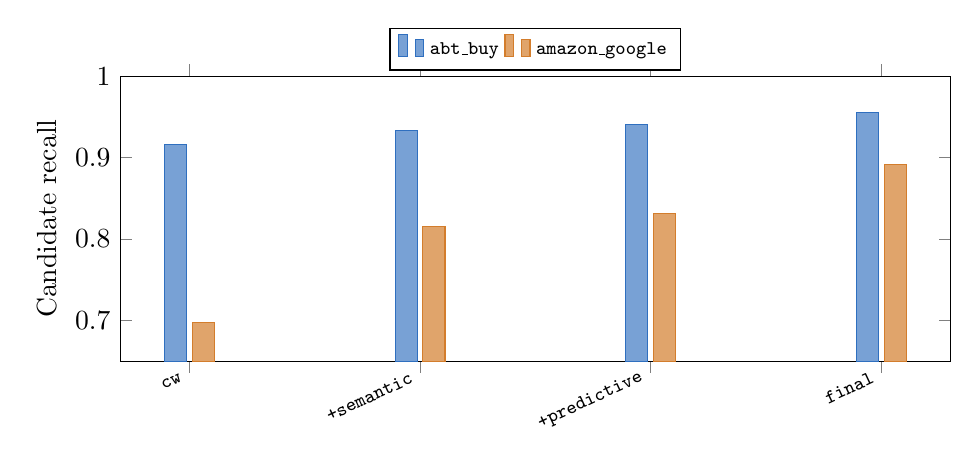
\begin{tikzpicture}
\begin{axis}[
  width=\columnwidth, height=5.2cm,
  ybar, bar width=8pt,
  symbolic x coords={cw, cw\_sem, cw\_sem\_pred, final},
  xtick=data,
  ymin=0.65, ymax=1.0,
  legend style={font=\scriptsize, at={(0.5,1.02)},
    anchor=south, legend columns=2},
  ylabel={Candidate recall},
  xticklabel style={rotate=25, anchor=east, font=\scriptsize},
  xticklabels={\texttt{cw}, \texttt{+semantic},
               \texttt{+predictive}, \texttt{final}}
]
\addplot[draw=recallblue,   fill=recallblue!65]
  coordinates {(cw,0.916)(cw\_sem,0.933)(cw\_sem\_pred,0.941)(final,0.955)};
\addplot[draw=precisionorange, fill=precisionorange!70]
  coordinates {(cw,0.698)(cw\_sem,0.815)(cw\_sem\_pred,0.831)(final,0.892)};
\legend{\texttt{abt\_buy}, \texttt{amazon\_google}}
\end{axis}
\end{tikzpicture}
\caption{Ablation: candidate recall as rescue phases are progressively added.
  Gains are gradual and consistent across both benchmarks.}
\label{fig:ablationgraph}
\end{figure}

\begin{table}[t]
\centering
\caption{Candidate-generation ablation results. \emph{Reduction} denotes the
  fraction of the Cartesian product avoided.}
\label{tab:ablation}
\small
\begin{tabular}{lccc}
\toprule
Strategy & Candidates & Recall & Reduction \\
\midrule
\multicolumn{4}{l}{\textit{\texttt{abt\_buy}}} \\
\texttt{cw}                  & 4,110  & 0.916 & 0.9965 \\
\texttt{cw\_semantic}        & 4,496  & 0.933 & 0.9962 \\
\texttt{cw\_sem\_predictive} & 4,576  & 0.941 & 0.9961 \\
\texttt{final verified}      & 5,733  & 0.955 & 0.9951 \\
\midrule
\multicolumn{4}{l}{\textit{\texttt{amazon\_google}}} \\
\texttt{cw}                  & 8,088  & 0.698 & 0.9982 \\
\texttt{cw\_semantic}        & 9,191  & 0.815 & 0.9979 \\
\texttt{cw\_sem\_predictive} & 9,330  & 0.831 & 0.9979 \\
\texttt{final verified}      & 12,349 & 0.892 & 0.9972 \\
\bottomrule
\end{tabular}
\end{table}

Figure~\ref{fig:ablationgraph} and Table~\ref{tab:ablation} trace the
evolution of candidate recall as rescue phases are added. Three observations
stand out:
\begin{enumerate}
  \item Pure symbolic witnesses already achieve strong reduction (>99.6\%),
    but recall is insufficient on noisy titles.
  \item Semantic rescue yields the largest single gain, focusing work only on
    symbolically weak entities.
  \item Predictive and bounded rescues provide further consistent improvement
    at modest candidate cost.
\end{enumerate}

The gradual, consistent gains across both benchmarks support the
interpretation that the final strategy emerged from measurable incremental
improvements rather than one lucky heuristic.

\subsection{Candidate Generation Results}

\begin{figure}[t]
\centering
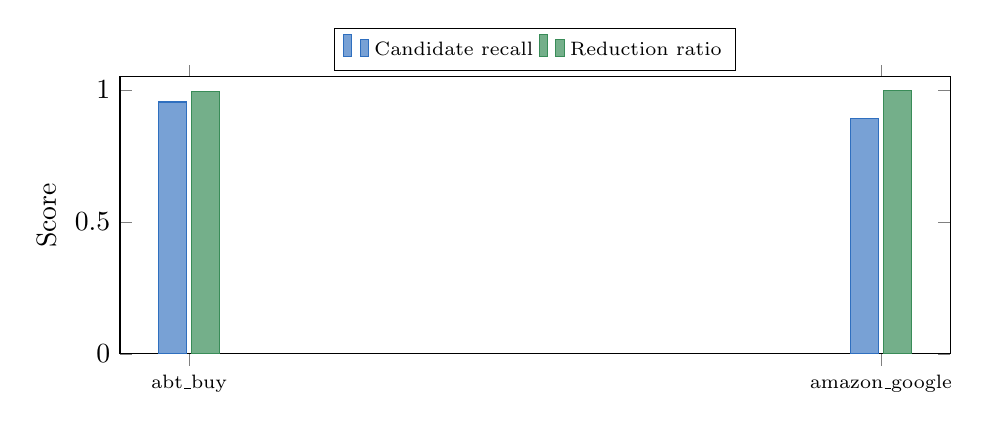
\begin{tikzpicture}
\begin{axis}[
  width=\columnwidth, height=5.1cm,
  ybar, bar width=10pt,
  symbolic x coords={abt\_buy, amazon\_google},
  xtick=data,
  ymin=0, ymax=1.05,
  legend style={font=\scriptsize, at={(0.5,1.02)},
    anchor=south, legend columns=2},
  ylabel={Score},
  xticklabel style={font=\scriptsize}
]
\addplot[draw=recallblue,     fill=recallblue!65]
  coordinates {(abt\_buy,0.955)(amazon\_google,0.892)};
\addplot[draw=reductiongreen, fill=reductiongreen!70]
  coordinates {(abt\_buy,0.9951)(amazon\_google,0.9972)};
\legend{Candidate recall, Reduction ratio}
\end{axis}
\end{tikzpicture}
\caption{Final candidate-generation results. Both datasets remain above 99\%
  reduction while candidate recall is sufficient for competitive end-to-end
  quality.}
\label{fig:candidategraph}
\end{figure}

\begin{table}[t]
\centering
\caption{Final candidate-generation results (current verified strategy).}
\label{tab:candidates}
\small
\begin{tabular}{lrrr}
\toprule
Dataset & Candidates & Recall & Reduction \\
\midrule
\texttt{abt\_buy}       & 5,733  & 0.955 & 0.9951 \\
\texttt{amazon\_google} & 12,349 & 0.892 & 0.9972 \\
\bottomrule
\end{tabular}
\end{table}

Table~\ref{tab:candidates} and Figure~\ref{fig:candidategraph} confirm the
core design claim: strong symbolic reduction followed by bounded rescue
preserves a high fraction of true matches while eliminating more than 99\%
of the Cartesian product.

\subsection{End-to-End Results}

\begin{figure}[t]
\centering
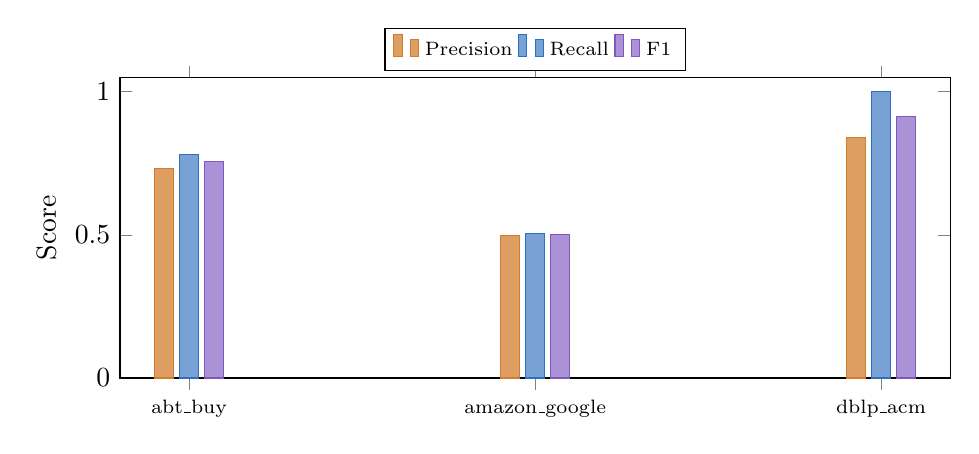
\begin{tikzpicture}
\begin{axis}[
  width=\columnwidth, height=5.4cm,
  ybar, bar width=7pt,
  symbolic x coords={abt\_buy, amazon\_google, dblp\_acm},
  xtick=data,
  ymin=0, ymax=1.05,
  legend style={font=\scriptsize, at={(0.5,1.02)},
    anchor=south, legend columns=3},
  ylabel={Score},
  xticklabel style={font=\scriptsize}
]
\addplot[draw=precisionorange, fill=precisionorange!75]
  coordinates {(abt\_buy,0.7312)(amazon\_google,0.4992)(dblp\_acm,0.8414)};
\addplot[draw=recallblue, fill=recallblue!65]
  coordinates {(abt\_buy,0.7812)(amazon\_google,0.5062)(dblp\_acm,0.9991)};
\addplot[draw=fiviolet, fill=fiviolet!65]
  coordinates {(abt\_buy,0.7554)(amazon\_google,0.5027)(dblp\_acm,0.9135)};
\legend{Precision, Recall, F1}
\end{axis}
\end{tikzpicture}
\caption{End-to-end precision, recall, and F1 on the three main benchmarks.
  \texttt{dblp\_acm} is structurally cleaner; \texttt{amazon\_google} is the
  most ambiguous.}
\label{fig:finalgraph}
\end{figure}

\begin{table}[t]
\centering
\caption{End-to-end results of the complete pipeline.}
\label{tab:finalresults}
\begin{tabular}{lccc}
\toprule
Dataset & Precision & Recall & F1 \\
\midrule
\texttt{abt\_buy}       & 0.7312 & 0.7812 & 0.7554 \\
\texttt{amazon\_google} & 0.4992 & 0.5062 & 0.5027 \\
\texttt{dblp\_acm}      & 0.8414 & 0.9991 & 0.9135 \\
\bottomrule
\end{tabular}
\end{table}

Table~\ref{tab:finalresults} and Figure~\ref{fig:finalgraph} present the
final end-to-end results. Three patterns stand out:

\textbf{\texttt{dblp\_acm}} achieves the best results (F1 = 0.9135) because
bibliographic records share strong and consistent title/author evidence.
Witness collapse is near-perfect on this dataset.

\textbf{\texttt{abt\_buy}} reaches a solid F1 of 0.7554. The dataset is
ambiguous enough that simple blocking fails, but compact product codes make
witnesses highly discriminative.

\textbf{\texttt{amazon\_google}} is the hardest benchmark (F1 = 0.5027).
Catalog descriptions vary significantly between Amazon and Google, making
symbolic evidence weaker and forcing the pipeline to rely more on semantic
rescue. The precision/recall gap is also smaller, suggesting the remaining
errors are genuinely hard cases.

\subsection{Comparison with PyJedAI}

PyJedAI~\cite{pyjedai} is an open-source ER framework providing strong
baseline implementations of blocking, matching, and clustering pipelines,
including pre-trained transformer-based matchers. Table~\ref{tab:external}
compares its reported numbers on the same benchmarks against our pipeline.

\begin{table}[h!]
\centering
\caption{Comparison with PyJedAI --- quality metrics (P, R, F1).}
\label{tab:external}
\small
\begin{tabular}{llcccc}
\toprule
System & Dataset & P & R & F1 & Time (s) \\
\midrule
Ours         & \texttt{abt\_buy}       & 0.7312 & 0.7812 & 0.7554 & 57.24  \\
PyJedAI      & \texttt{abt\_buy}       & 0.9617 & 0.8933 & 0.9263 & 16.91  \\
\midrule
Ours         & \texttt{amazon\_google} & 0.4992 & 0.5062 & 0.5027 & 144.13 \\
PyJedAI      & \texttt{amazon\_google} & 0.584  & 0.5615 & 0.5725 & 99.60  \\
\midrule
Ours         & \texttt{dblp\_acm}      & 0.8414 & 0.9991 & 0.9135 & 127.20 \\
PyJedAI      & \texttt{dblp\_acm}      & 0.9821 & 0.9883 & 0.9852 & 26.88  \\
\bottomrule
\end{tabular}

\vspace{0.8em}

\caption{Comparison with PyJedAI --- efficiency metrics (Reduction, Candidates, Total Pairs, Time).}
\label{tab:external2}
\small
\begin{tabular}{llccc}
\toprule
System & Dataset & Reduction & Candidates & Total Pairs \\
\midrule
Ours         & \texttt{abt\_buy}       & 0.9951 & 5,733  & 1,180,452 \\
PyJedAI      & \texttt{abt\_buy}       & 0.9950 & 5,895  & 1,180,452 \\
\midrule
Ours         & \texttt{amazon\_google} & 0.9972 & 12,349 & 4,397,038 \\
PyJedAI      & \texttt{amazon\_google} & 0.9967 & 14,436 & 4,397,038 \\
\midrule
Ours         & \texttt{dblp\_acm}      & 0.9981 & 11,183 & 6,001,104 \\
PyJedAI      & \texttt{dblp\_acm}      & 0.9980 & 11,803 & 6,001,104 \\
\bottomrule
\end{tabular}
\end{table}

PyJedAI outperforms our system across all datasets, particularly on
\texttt{amazon\_google}. The performance gap has two primary explanations.

First, PyJedAI uses transformer-based dense retrieval for candidate
generation, which provides much broader semantic coverage than our symbolic
witnesses. This is especially beneficial on noisy product titles where
token-level matching is fragile. Our system deliberately avoids this step
to remain CPU-first.

Second, PyJedAI employs pre-trained fine-tuned matchers, whereas our Step
3 uses a fixed multi-view scorer without fine-tuning. Fine-tuning on
labeled benchmark data substantially improves precision on hard cases.

The results show that our witness-driven system provides a practical CPU-first
alternative with competitive reduction ratios and respectable recall, and is
particularly effective on structured datasets like \texttt{dblp\_acm}. The
\texttt{amazon\_google} gap reflects the inherent difficulty of noisy
product matching without dense retrieval.

\subsection{Failure Analysis}

The remaining false negatives are no longer dominated by one failure pattern,
which is itself a positive sign. Analysis of residual errors identifies four
main hard-case types:
\begin{itemize}
  \item \emph{Title-poor vs.\ description-rich records}: one entity has
    a short title with weak token overlap.
  \item \emph{Generic catalog titles vs.\ SKU-rich titles}: no shared
    discriminative token exists.
  \item \emph{Software/version/edition drift}: version numbers differ
    between sources.
  \item \emph{Publisher or wrapper noise}: identical core content but
    different packaging in the catalog record.
\end{itemize}

The heterogeneity of these error types explains why each additional rescue
layer yields diminishing returns. Once the easy cases are resolved, the
remaining misses require increasingly specialised evidence that does not
generalise across benchmarks.

\subsection{Threats to Validity}

Three limitations should be kept in mind when interpreting the results.

\begin{enumerate}
  \item End-to-end experiments were not run in a single uniform batch; some
    measurements reflect iterative development over time rather than a
    controlled experimental sweep.
  \item Matching thresholds were not systematically re-calibrated per dataset;
    a global threshold may sub-optimally trade off precision and recall on
    specific benchmarks.
  \item The PyJedAI comparison relies on reference numbers from project
    documentation rather than a controlled head-to-head run under identical
    conditions.
\end{enumerate}

\section{Conclusion}

This project produced a complete, modular ER pipeline and a meaningful
research contribution in witness-driven candidate reduction. The practical
outcome is a four-stage architecture that supports multiple dataset formats,
transparent intermediate artifacts, resumable matching, and CPU-first
execution. The research contribution is the \texttt{cw\_semantic\_predictive}
strategy, which delays pair enumeration by reasoning over symbolic evidence
regions and applies bounded semantic rescue only where necessary.

Experiments on three standard benchmarks confirm the core claim: candidate
recall above 89\% with more than 99\% reduction of the Cartesian product,
and competitive end-to-end F1 scores without GPU inference. The
\texttt{dblp\_acm} benchmark (F1 = 0.9135) shows that the system performs
strongly when entity descriptions contain discriminative structured signals.
The \texttt{amazon\_google} gap relative to PyJedAI (0.5027 vs.\ 0.5725)
identifies dense retrieval as the main remaining lever for future work.

Key engineering lessons from the project:
\begin{itemize}
  \item Candidate recall is the most sensitive determinant of end-to-end
    quality; improvements at Step 2 amplify downstream.
  \item Monotone reranking is safer than subtractive collective evidence on
    noisy benchmarks.
  \item Strict empirical rollback discipline---removing any rescue that
    degraded the verified baseline---was essential for keeping the final
    system honest.
  \item Identifier hygiene and correct cross-source ID management matter as
    much as algorithmic design.
\end{itemize}

Future directions include threshold calibration per benchmark, lightweight
learned blocking to close the gap with dense-retrieval systems, and a
systematic visualisation of the reduction-versus-quality tradeoff across
the full dataset portfolio.

\section*{AI Assistance}
Large language models (Claude, Anthropic) were used as programming assistants
during this project. Specific uses included code review, CLI tooling
improvements, repository cleanup, and feedback on written sections.
The present report was also reviewed and corrected by a large language model,
which assisted with structure, clarity, consistency, and language quality.
All implementation decisions, experimental choices, evaluation, and final
project conclusions were made and verified by the team.

\begin{thebibliography}{9}
\bibitem{christophides2021survey}
V. Christophides, V. Efthymiou, T. Palpanas, G. Papadakis, and K. Stefanidis,
``End-to-End Entity Resolution for Big Data: A Survey,''
\emph{ACM Computing Surveys}, vol.~53, no.~6, 2021.

\bibitem{papadakis2016blocking}
G. Papadakis, J. Svirsky, A. Gal, and T. Palpanas,
``Comparative Analysis of Approximate Blocking Techniques for Entity
Resolution,''
\emph{Proceedings of the VLDB Endowment}, vol.~9, no.~9, 2016.

\bibitem{salton1988term}
G. Salton and C. Buckley,
``Term-Weighting Approaches in Automatic Text Retrieval,''
\emph{Information Processing and Management}, vol.~24, no.~5, 1988.

\bibitem{pyjedai}
K. Th. Nikoletos, G. Papadakis, and M. Koubarakis,
``pyJedAI: A Python Library for Explainable Entity Resolution,''
\emph{Proc. ISWC}, 2023.
\end{thebibliography}

\end{document}